% \begin{multicols}{2}

\subsection*{Verbundentropie}
\[
    H(a_i, a_j) = -\sum_{i=1}^{I} \sum_{j=1}^{J} \bigg[ P(a_i, a_j) \cdot
    \log_2( P(a_i, a_j) ) \bigg] \mbox{ [Bit]}
\]
\begin{itemize}
    \setlength{\parskip}{0pt}
    \setlength{\itemsep}{0pt plus 1pt}
    \item Einfachere Berechnung bei $P(a_i, a_j) = \frac{m_{ij}}{c}$:
\end{itemize}
\[
    H(a_i, a_j) = \frac{c \cdot \log(c) - \sum\limits_{i=1}^{I} \sum\limits_{j=1}^{J} \bigg[
    m_{ij} \cdot \log( m_{ij} ) \bigg]}{c \cdot \log(2)} \mbox{ [Bit]}
\]

\subsection*{Bedingte Entropie}
\[
    H(a_i | a_j) = - \sum_{i=1}^{I} \sum_{j=1}^{J} \bigg[ P(a_i, a_j)
    \log_2(P(a_i | a_j)) \bigg] \mbox{ [Bit]}
\]

\subsection*{Beziehungen zw.\ den Entropien}
\[
    H(a_i, a_j) = H(a_i | a_j) + H(a_j)
\]

\subsection*{Datenrate eines Kanals}
\[
    C = 2 \cdot B \cdot \log_2(L) \mbox{ [Bit/s]}
\]
\begin{itemize}
    \setlength{\parskip}{0pt}
    \setlength{\itemsep}{0pt plus 1pt}
    \item mit Anzahl der unterschiedlichen Amplituden $ L $
\end{itemize}
\[
    C = B \cdot \log_2 \left( 1 + \frac{S}{N} \right) 
\]
für $ \frac{S}{N} \ll 1 $:
\[
    C \approx 1.44 \cdot \frac{B}{\text{Hz}} \cdot \frac{S}{N} \mbox{ [Bit/s]}
\]
für $ \frac{S}{N} \gg 1 $:
\[
    C \approx 0.332 \cdot \frac{B}{\text{Hz}} \cdot \frac{SNR}{\text{dB}}
\]

\subsection*{Kanalkapazität}
\[
    C = \max_{P(a_k)} \bigg[ T(X; Y) \bigg]
\]

\subsection*{Transinformation}
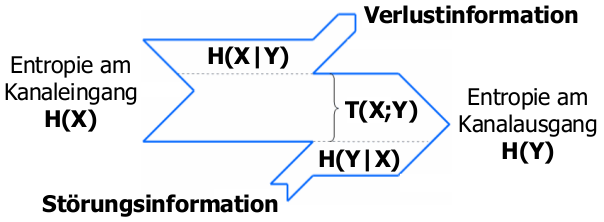
\includegraphics[width=0.5\textwidth]{transinformation}
\[
    T(X; Y) = H(X) - H(X | Y) = H(Y) - H(Y | X) = T(Y; X)
\]
Kanal ist 
\begin{itemize}
    \setlength{\parskip}{0pt}
    \setlength{\itemsep}{0pt plus 1pt}
    \item \textit{verlustfrei}, wenn Verlustinformation $ H(X | Y) = 0. $ \\
        $ \rightarrow C $ ist maximal, wenn alle Eingangssym.\ gleich
        wahrscheinlich
    \item \textit{deterministisch}, wenn Störungsinformation $ H(Y | X) = 0. $ \\
        $ \rightarrow C $ ist maximal, wenn alle Ausgangssym.\ gleich
        wahrscheinlich
    \item \textit{ungestört}, wenn er sowohl verlustfrei als auch
        deterministisch ist \\
        $ \rightarrow C $ ist maximal, wenn alle Ausgangssym.\ gleich
        wahrscheinlich oder alle Eingangssym.\ gleich wahrscheinlich
\end{itemize}

\subsection*{Theorem der Kanalcodierung}
Wenn $ H' \leq C' $ gilt, dann existiert immer eine Kanalcodierung, welche eine
Übertragung der Quellensymbole mit beliebig kleiner Fehlerwahrscheinlichkeit
ermöglicht (u.\ U.\ nur mit großem Aufwand).

\subsection*{Kraft'sche Ungleichung}
Für einen eindeutigen, binären Code mit $ K $ Codewörtern der Länge $ m_k $ gilt:
\[
    \sum_{k=1}^{K} 2^{-m_k} \le 1
\]

\subsection*{Theorem der Quellencodierung}
Die mittlere Länge $ \overline{m} $ eines Präfixcodes kann stets so gewählt
werden, dass gilt:
\[
    H \leq \overline{m} < H + 1
\]
Beim Huffman-Code:
\[
    H \leq \overline{m} < H + p_{\max} + 0.086
\]
bzw.\ wenn $ p_{\max} > 0.5 $:
\[
    H \leq \overline{m} < H + p_{\max}
\]

% \end{multicols}
